% !TeX root = ../main.tex
\clearpage
\pagestyle{plain}
\addcontentsline{toc}{chapter}{Prelude}
\begin{center}
	{\textbf{\Large Prelude}}
\end{center}

\begin{center}
	\includegraphics[width=.5\textwidth]{images/intro/sea_hath_its_pearls.jpg}

	\vspace{1em}
	{William Henry Margetson, \textit{The Sea Hath its Pearls} (1897).}
\end{center}

From UC Santa Cruz's Engineering 2 Building, where much of the work in this thesis had its genesis, it is a one mile walk through a shaded redwood forest to East Field, where the trees give way to a large sloping meadow looking out over Santa Cruz and the entire Monterey Bay. It is here I often went to think through a hard problem, or just to get away from the computer screen and let my mind settle. %And while this thesis is focused on validating the correctness and security of concurrent shared-memory behavior on GPUs, it seems apt to use UC Santa Cruz's proximity to a place as impressive as the Monterey Bay to create a metaphor between it and the research presented here.

Viewed from the vantage point of East Field, 600 feet up, the Pacific Ocean often looks calm and empty, with only the afternoon whitecaps hinting that its peaceful veneer is nothing more than a facade. Because in fact, the Monterey Bay teeming with life; it is one of the most biodiverse environments on Earth, and its opaque surface hides from view the deepest submarine canyon on the North American coast, with walls plunging over a mile down into the depths. Deep down, wild sea creatures live, including predators like the Black Seadevil Anglerfish. This fish has only been filmed alive at depth twice, with one of those observations occurring in 2014 in the Monterey Bay Canyon itself.

\begin{center}
	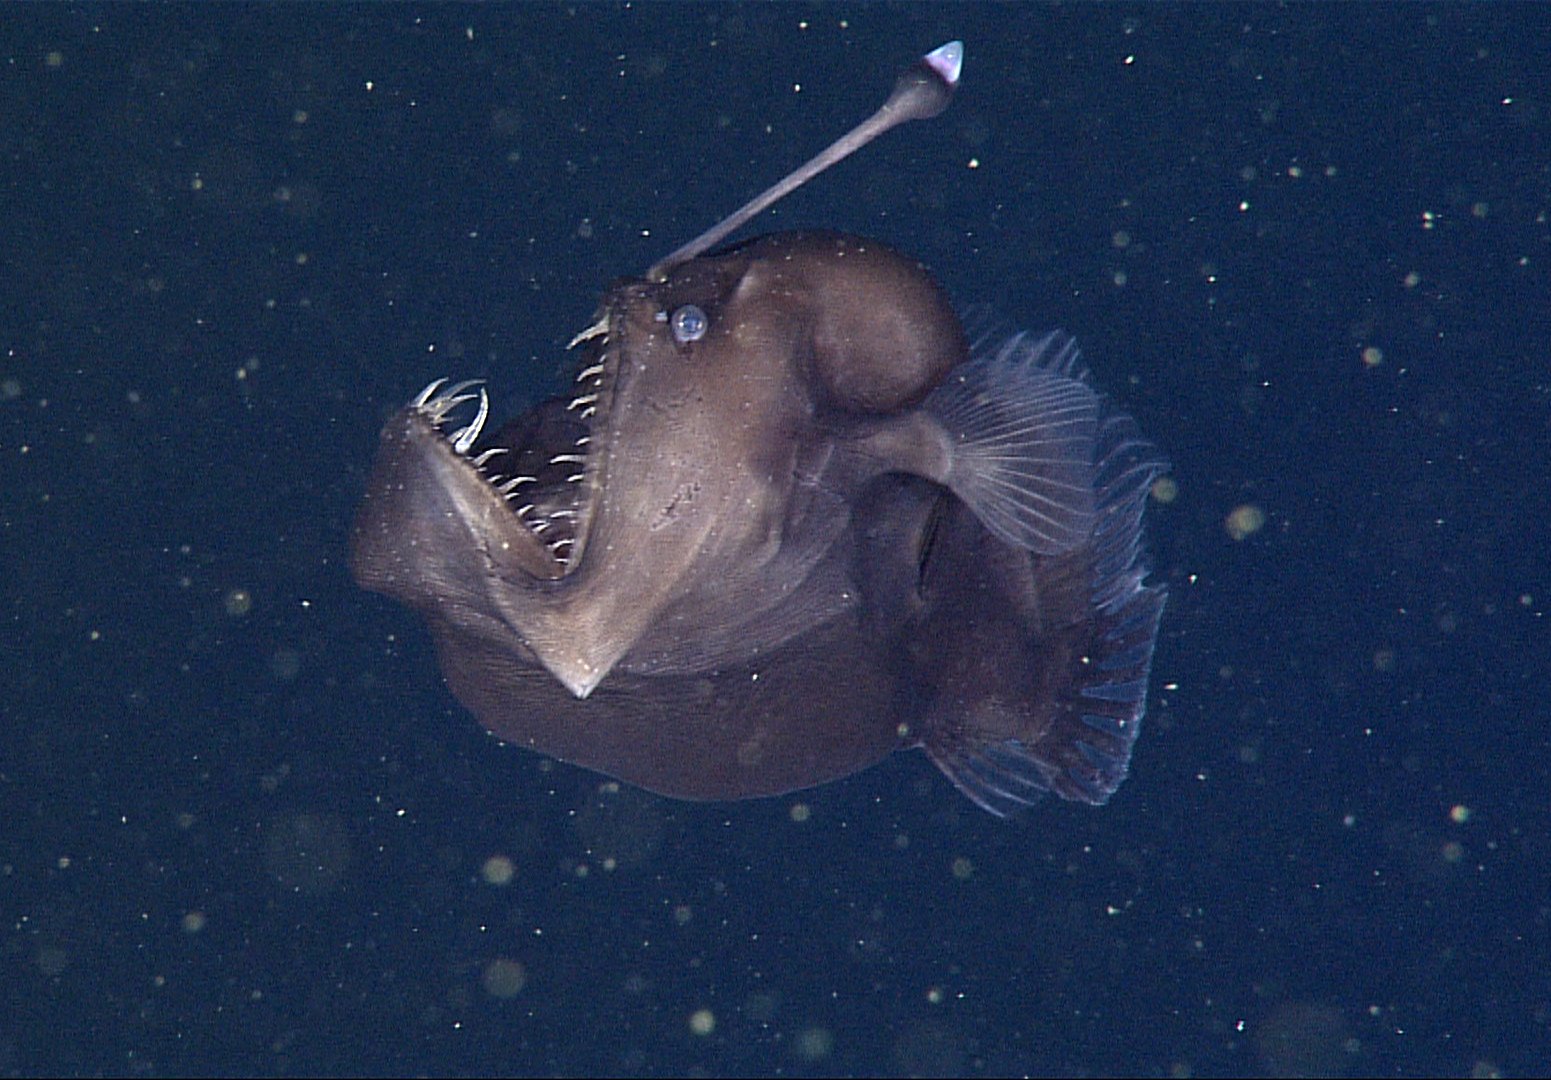
\includegraphics[width=.7\textwidth]{images/intro/sea_devil.jpg}

	\vspace{1em}
	{The sea hath its devils. MBARI, 2014.}
\end{center}

A trip to the tidepools at Natural Bridges State Beach or a whale watching boat tour are great ways to sample the Monterey Bay and leave one awe-inspired, but these experiences only give a glimpse into the complex and ever-changing environment that lies below. For it is the submarine canyon itself that is responsible for the Monterey Bay's incredible biodiversity, as ocean currents interact with the canyon's geography to bring cold, nutrient-rich water closer to the surface. From the hermit crab scuttling across the rocky reefs, to the sea otters wrapped securely in the kelp forests just offshore, to the orca pods patrolling the edges of the submarine canyon, all of the visible wonders ultimately depend on the upwellings from the hidden submarine canyon.


Similarly, this thesis is an exploration into the depths of GPU programming models, investigating the relatively little-understood concurrent shared-memory behaviors of modern GPU hardware and their software stacks. Just as the Monterey Bay submarine canyon is responsible for upholding its entire ecosystem, correct specifications and implementations of concurrent shared-memory provide the backbone that modern GPU applications are built on. So, whether it's pearls or seadevils that we find, I invite you to dive into the depths of GPU programming models with me now, and I hope you come away at least slightly more informed and inspired by the sophisticated parallel processors that power so many of today's most important applications.

\clearpage
